A Consideration of Towering Scheme for Efficient Arithmetic Operation over Extension Field of Degree 18

Barreto-Naehrig (BN) curve is a well studied pairing friendly curve of embedding degree 12, that uses arithmetic in $\FQTV$. Therefore the arithmetic of $\FQTV$ extension field is well studied. In this thesis, we have proposed an efficient approach of arithmetic operation over the extension field of degree 18 by towering. $\FQEN$ extension field arithmetic is considered to be the basis of implementing the next generation pairing based security protocols. We have proposed to use $\FQ$ element to construct irreducible binomial for building tower of extension field up to $\FQSX$, where conventional approach uses the root of previous irreducible polynomial to create next irreducible polynomials. Therefore using $\FQ$ elements in irreducible binomial construction, reduces the number of multiplications in $\FQ$ to calculate inversion and multiplication over $\FQEN$, which effects acceleration in total arithmetic operation over $\FQEN$.



\section{Introduction}
The emerging information security of computer system stands on the strong base of cryptography. Compared to RSA cryptography, elliptic curve cryptography \cite{koblitz1987elliptic} gained much attention for its faster key generation, shorter key size with same security level and less memory and computing power consumption. Intractability of Elliptic Curve Discrete Logarithm Problem (ECDLP) encourages many innovative cryptographic protocols. At the very beginning of the twenty first century, a cyptosystems based on elliptic curve pairing was proposed independently by Sakai et al. \cite{EPRINT:SakKas03} and Joux \cite{JC:Joux04}. Since then this pairing based cryptosystem has unlocked several novel ideas to researchers such as Identity based encryption scheme explained by Boneh et al. \cite{C:BonFra01}. In addition, group signature authentication \cite{C:BonBoySha04},\cite{AC:NakFun05} and broadcast encryption \cite{C:BonGenWat05} has increased the popularity of pairing based cryptography. Pairings such as Weil\cite{Weil_p}, Tate and Optimal-ate \cite{DBLP:journals/tit/Vercauteren10}, Eta \cite{IEEETIT:HesSmaVer06} and $\chi$-Ate \cite{PAIRING:NASKM08} pairings has gained much attention in recent years. Pairing is a bilinear map from two rational point groups denoted by $\g1$ and $\g2$ to a multiplicative group denoted by $\g3$ \cite{Silverman}. It is generally denoted by $\g1 \times \g2 \rightarrow \g3$. In addition, these groups are defined over a certain extension field $\FQK$, where $p$ is the prime number, also called characteristics  and $k$ is the extension degree, especially called \textit{embedding} degree. 
Therefore it is important to efficiently construct extension field arithmetic in order to make pairing based cryptography efficient.

In prairing based cryptography, rational points are defined over a certain pairing friendly elliptic curve. Let $E(\FQK)$ be a set of rational points such as $(x, y)$,  $x, y \in \FQK$ lies in the elliptic curve $E$, defined over extension field $\FQK$ of embedding degree $k$. Security level of pairing based cryptography depends on the sizes of both $r$ and $p^k$, where $r$ denotes the largest prime number that divides the order of $E(\FQ)$. It is said that the next generation pairing-based cryptography needs $\log_2 r \approx 256$ and $\log_2 p^k \approx 3000$ to $5000$. Supposing the most efficient case of $\rho = (\log_2 p)/(\log_2 r) = 1$, $k$ needs to be $12$ to $20$.  In this thesis we are considering $k=18$ and $18$ degree pairing friendly curve described in \cite{EPRINT:FreScoTes06}. 

While using pairing based protocols, it is required to perform arithmetic in higher fields, such as $\FQK$  for moderate value of $k$ \cite{Silverman}. It is important to represent the field in such a way that, the arithmetic can be performed efficiently.  One of the most efficient way is to use the tower of extension field \cite{EPRINT:BenSco09}. Which explains that, higher level computations can be calculated as a function of lower level computations. Because of that, efficient implementation of lower level arithmetic results in the good performance of arithmetic in higher degree fields. Recently the implementation of pairing based cryptosystems for different low power and mobile devices are increasing. Moreover, the hardware capabilities of the embedded devices are improving which can make pairing implementations efficient and faster. Therefore efficiency of extension field arithmetic is important to improve the performance of pairing. In this thesis we have presented an efficient way to construct $\FQEN$  extension field and performing arithmetic operation on that field. In current approach of constructing extension field by towering, root of previous irreducible polynomial is used to construct the irreducible polynomial for next extension field. In our proposal, element in prime field $\FQ$ is used to construct the irreducible polynomial for the first two extension field and for in the last extension field root of base extension field is used for constructing irreducible polynomial.


\section{Preliminaries}
In this section we will go though the background how tower of extension field is constructed in practice and some basic idea of basis to construct extension field. 
\subsection{Basis of extension field and towering}
In order to construct the arithmetic operations in $\FQK$, we generally need an irreducible polynomial $f(x)$ of degree $k$ over $\FQ$. Let $\omega$ be a zero of $f(x)$, that is $\omega \in \FQK$, then the following set forms a basis of  $\FQK$ over $\FQ$
\begin{equation}\label{basis_fpm}
\left\lbrace 1, \omega, \omega^2 , \cdots, \omega^{k-1} \right\rbrace,
\end{equation}
which is known as polynomial basis. An arbitrary element $A$ in  $\FQK$ is written as
\begin{equation}\label{element_fpm}
A = a_0 +a_1\omega + a_2\omega^2 + \cdots + a_{k-1}\omega^{k-1}. 
\end{equation}
The vector representation of $A$ is   $v_A =(a_0, a_1, a_2, \cdots a_{k-1})$. Multiplication and inversion in  $\FQK$ are carried out by using the relation $f(\omega) = 0$, and therefore $f(x)$ is called the \textit{modular reduction polynomial} of  $\FQK$. Frobenious mapping should be efficient while calculating conjugates of $\omega$. 

Extension field of $\FQK$ with moderate value of $k$, such as $k \geq 6$ needs to be represented as a tower of sub extension field to improve pairing calculation. In \cite{lane2008draft}  explained tower of extension by using irreducible binomial. In case of Barreto-Naehrig (BN) curves  \cite{SAC:BarNae05}, where $k=12$, towering extension field with irreducible binomial is represented as follows:
\begin{equation}\label{eq:BN_towering}
\begin{cases}
\F{p}{2} = \F{q}{}[\omega]/(\omega^2-\beta), \mbox{where $\beta = c$ and $c \in \FQ$}.\nonumber \\ 
\F{p}{6} = \F{q}{2}[\tau]/(\tau^3-\xi), \mbox{where $\xi = \omega+1$}.\nonumber \\ 
\F{p}{12} = \F{q}{6}[\theta]/(\theta^2-\tau),\mbox{where $\tau = \xi$}. \nonumber \\ 
\end{cases}
\end{equation}
Here $p$ needs to be prime and $p-1$ needs to be divisible by 4 and $c$ should be quadratic and cubic non residue over $\FQ$.

In this section we will construct the extension field of degree 18 as a tower of three sub extension field. The extension field $\FQTH$ is the sextic twist of $\FQEN$. Therefore its is considered as the base field for constructing $\FQTHTWTH$ extension field in our proposal. Figure \ref{fig_field} shows the top level overview of our proposal to construct the tower of extension fields.

\begin{figure*}
\centering
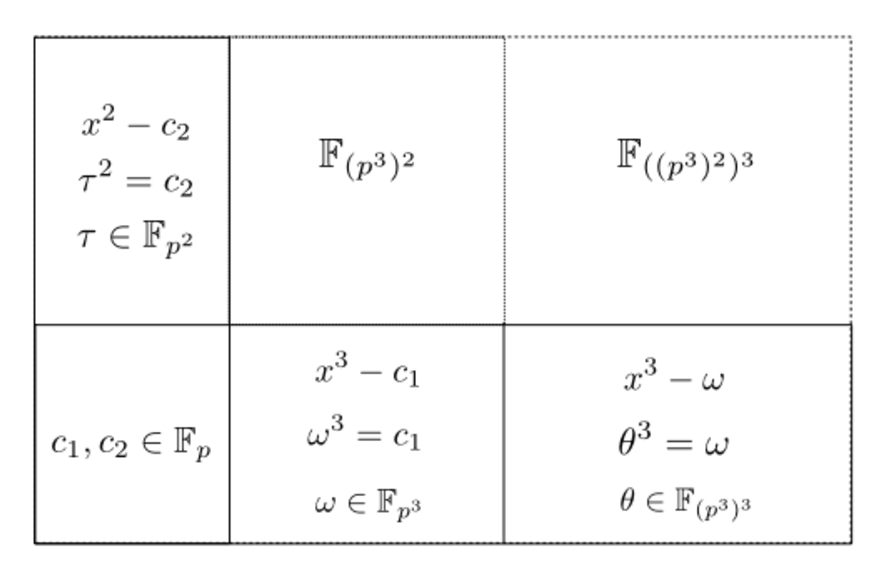
\includegraphics[width=7.5cm, height=4cm]{Field.eps}
\caption{Construction overview of $\FQTHTWTH$}
\label{fig_field}
\end{figure*}

\subsection{Arithmetic operations over extension field $\FQTH$}
At first, let us consider arithmetic operations in $\FQTH$, which is the degree $3$ extension field over $\FQ$. 
In order to perform arithmetic operations in $\FQTH$, we generally need an irreducible polynomial $f(x)$ of degree $3$ over $\FQ$. Specifically irreducible binomial is efficient to use as reduction modular polynomial. In order to obtain such binomial, Legendre symbol $\Leg{c_1}{p}$ is convenient.
Let us consider $3|(p-1)$ and a non-zero element $c_1 \in \FQ$. 
\begin{equation}\label{eq:legndre_3}
c_1^{\frac{p-1}{3}} = 
\begin{cases}
  0 \quad & \mbox{$c_1 = 0$},\\
  1 \quad &\mbox{CPR},\\
  otherwise & \mbox{CPNR},
\end{cases}
\end{equation}
where CPR and CPNR are abbreviations of cubic power residue and cubic power non residue, respectively. If $c_1$ does not have any cubic root in $\FQ$, $f(x) =x^3 - c_1$ becomes an irreducible binomial over $\FQ$. Let $\omega$ be a zero of $f(x)$, which is an element in $\FQTH$. Therefore the set $\left\lbrace 1, \omega, \omega^2 \right\rbrace $ forms a polynomial basis of $\FQTH$ over $\FQ$. Now let us consider two arbitrary element $\textbf{a, b}$ in $\FQTH$, can be represented as follows:
\begin{eqnarray}\label{eq:vec_A_Fq_3}
\textbf{a} & = & a_0 + a_1\omega+ a_2\omega^2,  \nonumber \\ 
\textbf{b} & = & b_0 + b_1\omega+ b_2\omega^2,  \nonumber \\
& & a_i, b_j \in \FQ .  \nonumber
\end{eqnarray} 

\subsubsection{Addition and subtraction in $\FQTH$}
Addition, subtraction within the elements and multiplication by a scalar with any element in $\FQTH$ are carried out by coefficient wise operations over $\f{p}$ as follows,
\begin{eqnarray}\label{eq:add_sub_fq3}
\textbf{a} \pm \textbf{b} & = &  (a_0 \pm b_0, a_1 \pm b_1, a_2 \pm b_2), \\
k\textbf{a} & = &  (ka_0,  ka_1,ka_2),  \mbox{ $k \in \FQ$}.
\end{eqnarray}

\subsubsection{Multiplication in $\FQTH$}
Multiplication of two arbitrary vectors is performed as follows:
%\begin{subequations}
\begin{eqnarray}
\textbf{ab} & = & (a_0 + a_1\omega+ a_2\omega^2)(b_0 + b_1\omega+ b_2\omega^2)\nonumber\\
& = & a_0 b_0 + (a_0 b_1+a_1 b_0)\omega + (a_0 b_2 +a_1 b_1 + a_2 b_0)\omega^2 \nonumber \\ 
&  & + (a_1 b_2+a_2 b_1)\omega^3 +a_2b_2\omega^4.  \label{eq:mul_fq3_a}
%& = &(a_0 b_0 + c_1 a_1 b_2 + c_1 a_2 b_1) + (a_0 b_1+ a_1 b_0 \nonumber \\
%& & + c_1 a_2 b_2)\omega + (a_0 b_2 +a_1 b_1 + a_2 b_0)\omega^2 \label{eq:mul_fq3_b}
\end{eqnarray}
%\end{subequations}
Here in \eqref{eq:mul_fq3_a}, there are 9 multiplications and 4 additions in $\FQ$. To reduce the number of multiplications in \eqref{eq:mul_fq3_a}, we apply Fast Polynomial Multiplication introduced in \cite{JC:BaiPaa01} as follows:
\begin{eqnarray}\label{eq:FPM}
A_0 & = & a_0b_0\nonumber \\
A_1 & = & a_1b_1\nonumber \\
A_2 & = & a_2b_2\nonumber \\
A_3 & = & (a_0+ a_1)(b_0+b_1)\nonumber \\
A_4 & = & (a_0+ a_2)(b_0+b_2)\nonumber \\
A_5 & = & (a_1+ a_2)(b_1+b_2), 
\end{eqnarray}
where $A_i, i= 0,1, \cdots, 5$ are the auxiliary products. Let us consider $\textbf{ab} = t(\omega) = \sum_{i=0}^{4} t_i\omega^i$.
Now we can represent the coefficients $t(\omega)$ as only additions and subtractions of  $A_i$,
\begin{eqnarray}\label{eq:FPM1}
t_0 & = & A_0\nonumber \\
t_1 & = & A_3 - A_1 - A_0 \nonumber \\
& = & (a_0b_0 +a_0b_1+a_1b_0+a_1b_1)-a_1b_1-a_0b_0 \nonumber \\
t_2 & = & A_4 - A_2 - A_0 + A_1\nonumber \\
& = & (a_0b_0 +a_2b_0+a_0b_2+a_2b_2)-a_2b_2-a_0b_0 +a_1b_1\nonumber \\
t_3 & = & A_5 - A_1 - A_2\nonumber \\
& = & (a_1b_1 +a_1b_2+a_2b_1+a_2b_2)-a_1b_1-a_2b_2 \nonumber \\
t_4 & = & A_2.
\end{eqnarray}
Considering subtractions as additions, from the above equations we find that only 6 multiplications and 13 additions are required in $\FQ$ for multiplying two arbitrary vectors in $\FQTH$. Therefore, compared to \eqref{eq:mul_fq3_a} the above method will accelerate the vector multiplication, since in most processors multiplication is slower than addition. Substituting $\omega^3 = c_1$ in \eqref{eq:mul_fq3_a}, owing to the fact that $f(\omega) = 0$ of the irreducible binomial $f(x)=x^3-c_1$; $\textbf{ab}$ becomes as follows:
\begin{eqnarray}\label{fq_3_t}
\textbf{ab} & = & t_0 + t_1\omega + t_2\omega^2 + t_3 \omega^3 + t_4\omega^4 \nonumber \\
& = & (t_0 + c_1 t_3 ) + (t_1+c_1 t_4)\omega + t_2\omega^2.
\end{eqnarray}
Here it requires 2 more $\FQ$ additions. Multiplication with  $c_1$  will not increase the number of multiplications in $\FQ$ since $c_1$ is small such as $2$ and it can be achieved using bit wise shifting. Finally 6 multiplications and 15 additions are required in $\FQ$ to multiply two elements in $\FQTH$.

\subsubsection{Squaring in $\FQTH$}
Squaring of an $\FQTH$  element $A$ is performed by applying Chung-Hasan method \cite{chung2007asymmetric} as following.

\begin{eqnarray}\label{chung_h}
A^2 & = & (a_0 + a_1\omega + a_2\omega^2)^2 \nonumber\\
& =  & a_0^2 +2c_1a_1a_2 +[2a_0a_1 +c_1a_2^2]\omega+[(a_0 +a_1 +a_2)^2 \nonumber \\
&&-(a_0^2 + a_2^2 + 2a_1a_2 + 2a_0a_1)]\omega^2.
\end{eqnarray}
In what follows, let us consider \eqref{chung_h} be written as $\textbf{AB} = S_1 +S_2\omega + S_3\omega^2$ and  the coefficients are expressed as \eqref{sq_sub}. The following terms can be pre-calculated to reduce the number of operations. $ T_1= 2a_1$, $T_2 = a_0^2$, $T_3=a_2^2$, $T_4=T_1a_2$, $T_5=T_1a_0$, $T_6 = (a_0+a_1+a_2)^2$.
\begin{subequations} \label{sq_sub}
\begin{eqnarray}
S_1 & = & T_2+c_1T_4, \\
S_2 & = & T_5+c_1T_3,\\
S_3 & = & T_6 - (T_2+T_3+T4+T_5).
\end{eqnarray}
\end{subequations}
When $c_1 = 2$ , the operation cost of a squaring in $\FQTH$ is 2 multiplications, 3 squaring and 8 additions in $\FQ$ and 2 bit wise left shifting.
\subsubsection{Vector inversion in $\FQTH$}
The inverse element $\textbf{a}^{-1} \in \F{p}{3}$, can be easily calculated using Frobenius mapping (FM) $\pi(\textbf{a})$. At first we find the conjugates $\textbf{a}^p$, $\textbf{a}^{p^2}$ of $\textbf{a}$ by applying FM. Then the inverse element $\textbf{a}^{-1}$  is calculated as follows.
\begin{equation}
\textbf{a}^{-1} = n(\textbf{a})^{-1}(\textbf{a}^p\textbf{a}^{p^2}), \label{Inv_Cal_fq3}
\end{equation}
where $n(\textbf{a})= (\textbf{a}\textbf{a}^{p}\textbf{a}^{p^2}) \in \mFp$ is the product of conjugates. Conjugate $\textbf{a}^p=  (a_0+a_1\omega+a_2 \omega^2)^p$ can be easily calculated as follows:
\begin{eqnarray}\label{eq:FM_aq}
(a_0+a_1\omega+a_2 \omega^2)^p& = & (a_0 + a_1 \omega)^p+ (a_2 \omega^2)^p\nonumber\\
& = & a_0+a_1(\omega^3)^{\frac{p-1}{3}}\omega  \nonumber \\ 
& & + a_2 ((\omega^3)^{\frac{p-1}{3}})^2 \omega^2  \nonumber \\ 
& = & a_0+a_1(c_1)^{\frac{p-1}{3}} \omega  \nonumber \\
& & + a_2 ((c_1)^{\frac{p-1}{3}})^2 \omega^2 \nonumber \\
& = & a_0 + a_1 c_1' \omega + a_2 c_1'' \omega^2 \nonumber \\
& = & a_0 + a_1' \omega + a_2' \omega^2,
\end{eqnarray}
where $a_1', a_2' \in \FQ$ and $c_1' = (c_1)^{\frac{p-1}{3}}$ is already known from \eqref{eq:legndre_3} and $c_1'' = (c_1')^2$ can be precalculated. In the above computation, 2 multiplications in $\FQ$ is required. 
Now the other conjugate $\textbf{a}^{p^2}$ can be calculated with the same number of operations according to the above procedure as follows:
\begin{eqnarray}
\textbf{a}^{p^2} & = & (\textbf{a}^p)^p\nonumber \\
& = &  (a_0 + a_1' \omega + a_2' \omega^2)^p\nonumber \\
& = & a_0 + a_1' c_1' \omega + a_2' c_1'' \omega^2 \nonumber \\
& = & a_0 + a_1'' \omega + a_2'' \omega^2,
\end{eqnarray} 
where $a_1'', a_2'' \in \FQ$.
Before calculating $n(\textbf{a})$ we first calculate the multiplication of $(\textbf{a}^p\textbf{a}^{p^2})$ like \eqref{eq:mul_fq3_a} as follows
\begin{eqnarray}\label{eq:mul_aq_aq2}
\textbf{a}^p\textbf{a}^{p^2} & = & (a_0 + a_1'\omega+ a_2'\omega^2)(a_0 + a_1''\omega+ a_2''\omega^2).
%& = & (a_0^2 + c_1a_1' a_2''+c_1a_2' a_1'') + (a_0 a_1' + a_0 a_1'' \nonumber \\
%& & +c_1a_2'a_2'')\omega + (a_0 a_2' +a_1' a_1'' + a_0 a_2'')\omega^2.
\end{eqnarray}
Now let us consider the following representation. \\ $\textbf{T}= \textbf{a}^p\textbf{a}^{p^2}  = (t_0,t_1,t_2), \quad  n(\textbf{a}) =s= \textbf{aT}$,\\
Thereby the inversion of $\textbf{a}$ can be expressed as $\textbf{a}^{-1}= s^{-1}\textbf{T}$.
The vector representation of the non-zero scalar $s$ is written as $s = (s,0,0)$. 
In addition, $\textbf{a}^p$ and $\textbf{a}^{p^2}$ is represented by the following equations by using the relation $c_1'^2+c_1'+1=0$, where $c_1'^3=1$.
\begin{subequations}
\begin{equation}
\textbf{a}^p  =  (a_0, c_1' a_1, c_1'^2 a_2)  =  (a_0, c_1'a_1,-a_2-c_1'a_2),
\end{equation}
\begin{equation}
\textbf{a}^{p^2} =  (a_0, c_1'^2 a_1, c_1' a_2)  =  (a_0, -a_1-c_1'a_1,c_1'a_2).
\end{equation}
\end{subequations}
Now let us consider the variables $T_0 \sim T_5$ as following expressions.
\begin{subequations}
\begin{eqnarray}
 T_0 & = & a_0^2,\nonumber \\
  T_1 & = & a_1^2, \nonumber \\
  T_2 & = & a_2^2, \nonumber \\
 T_3 & = & (c_1'a_1+c_1'^2a_2)(c_1'^2a_1+c_1'a_2)\nonumber \\
 &  = & a_1^2-a_1a_2+a_2^2\nonumber\\
 T_4 & = & (a_0+c_1'a_1)(a_0+c_1'^2a_1)\nonumber\\
 &= &a_0^2-a_0a_1+a_1^2\nonumber\\
 T_5 & = & (a_0+c_1'^2a_2)(a_0+c_1'a_2)\nonumber\\
 &= & a_0^2-a_0a_2+a_2^2.\nonumber
 \end{eqnarray}
\end{subequations}
The elements of $\textbf{T} = (t_0,t_1,t_2)$ can be obtained as follows:
\begin{subequations}
\begin{eqnarray}
t_1  & = &   T_0 + c_1 (T_3 - T_1 - T_2) \nonumber \\
& = & a_0^2 - c_1a_1a_2,\\
t_2 & = & T_4- T_0 - T_1 +c_1 T_2 \nonumber\\
& = & c_1a_2^2 - a_0a_1,\\
t_3 & = & T_5 -T_0 - T_2 +T_1 \nonumber \\
& = & a_1^2 - a_0a_2.
\end{eqnarray}
\end{subequations}
The calculation cost of $t_1,t_2,t_3$ is 3 multiplications, 3 squaring, 3 additions and 2 bit shifting. The vector multiplication for getting $s = \textbf{aT} =(s,0,0)$ can be done by calculating $s = a_0b_0+c_1(a_1b_2+a_2b_1)$ which costs 3 multiplication, 2 additions and 1 bit shifting. 

Finally the inversion of the scalar $s$ and multiplication by the inverse of scalar $s$ with vector $\textbf{T}= \textbf{a}^p\textbf{a}^{p^2}$ can be obtained by distributive law which takes 1 inversion and 3 multiplication in $\FQ$. Therefore the total cost of inversion is 9 multiplications, 3 squaring, 5 additions, 3 bit shifting and 1 inversion in $\Fp$. 

%This result can be saved for further use. Thus \eqref{eq:mul_aq_aq2} has 6 multiplications and 15 additions in $\FQ$ according to \eqref{eq:FPM} and \eqref{eq:FPM1}. Similarly multiplying $\textbf{a}$ with \eqref{eq:mul_aq_aq2} yields $n(\textbf{a})$ which will have no $\omega$ terms. That is $n(\textbf{a})$  will be a scalar. The total calculation cost for $n(\textbf{a})$ is 16 multiplications and 26 additions. Therefore the inversion of $\textbf{a} \in \FQTH$ can be easily calculated from \eqref{Inv_Cal_fq3} with 19 multiplications, 26 additions and 1 inversion in $\FQ$. 

\subsection{Arithmetic operations over extension field $\FQTHTW$}
$\FQTHTW$ is constructed with the irreducible binomial $g(x)=x^2-c_2$ where $c_2 \in \FQ$. Here it differs from the existing method to towering. Existing method uses $x^2-\omega$ as the irreducible polynomial in $\FQSX$; that is the root of irreducible binomial of $\FQTH$ is used to construct irreducible binomial in $\FQSX$. In this proposed approach, such binomial can be easily obtained by applying Legendre Symbol $\Leg{c_2}{p}$ over $\FQ$. Then let its zero be $\tau$,$\tau \in \FQTHTW$, therefore the set $\left\lbrace 1, \tau \right\rbrace $ forms the polynomial basis in $\FQTHTW$. If we choose $p$ such that $p \equiv 3$ (mod $4$), that will accelerate the arithmetic operation significantly; since multiplication by $c_2=-1$ will be calculated only by substitution. Let us consider $\textbf{m},\textbf{n}$ as two arbitrary elements in $\FQTHTW$ as follows:

\begin{eqnarray}\label{eq:vec_mn_Fp3_2}
\textbf{m} & = & \textbf{a}_0 + \textbf{a}_1\tau,  \nonumber \\ 
\textbf{n} & = & \textbf{b}_0+\textbf{b}_1 \tau,  \nonumber \\
& & \textbf{a}_i, \textbf{b}_j \in \F{p}{3}.  \nonumber
\end{eqnarray} 

Addition and Subtraction is done coefficient wise similar to those in $\FQTH$. Multiplication of $\textbf{m},\textbf{n}$ is done as follows:
\begin{eqnarray}\label{eq:mul__Fp_3_2}
\textbf{mn} & = & (\textbf{a}_0+\textbf{a}_1\tau)(\textbf{b}_0+\textbf{b}_1\tau)\nonumber\\
& = & \textbf{a}_0 \textbf{b}_0 + (\textbf{a}_0 \textbf{b}_1+\textbf{a}_1 \textbf{b}_0)\tau + \textbf{a}_1\textbf{b}_1\tau^2 \nonumber \\ 
& = &(\textbf{a}_0 \textbf{b}_0 + c_2 \textbf{a}_1 \textbf{b}_1)+ (\textbf{a}_0 \textbf{b}_1+\textbf{a}_1 \textbf{b}_0)\tau  \label{eq:mul_Fp_3_2a}\\ 
& = &(\textbf{a}_0 \textbf{b}_0 + c_2 \textbf{a}_1 \textbf{b}_1) + (\textbf{a}_0 +\textbf{a}_1)( \textbf{b}_0 +\textbf{b}_1)\tau \nonumber \\ 
&    &  - (\textbf{a}_0\textbf{b}_0)\tau - (\textbf{a}_1\textbf{b}_1)\tau.
\end{eqnarray}
Here Karatsuba method \cite{Karatsuba} is applied. In this calculation, we have substituted $\tau^2 = c_2$, as $\tau$ is a zero of the irreducible binomial $g(x)=x^2-c_2$. Since prime number $p$ is chosen such that $p \equiv 3$ (mod $4$), therefore $c_2$  is just substituted with $-1$. That means  multiplication with $c_2$ needs no countable computations in $\FQ$. Moreover multiplication of $\textbf{a}_1\textbf{b}_1$ and $\textbf{a}_0\textbf{b}_0$ will be reused. Therefore we need 3 multiplications and 5 additions in $\FQTH$ to multiply two vectors over $\FQTHTW$, where we consider subtractions as additions.

\subsubsection{Vector inversion in $\FQTHTW$}
For calculating the multiplicative inverse vector of a non-zero vector $\textbf{m}\in \FQTHTW$, first we calculate the conjugate of $\textbf{m}$ that is given by  Frobenius mapping  $\pi_{p^3}(\textbf{m}) = \textbf{m}^{p^3}$. Then the inverse of $\textbf{m}$, $\textbf{m}^{-1}$ is calculated as follows:
\begin{equation}\label{InvCal_fq_3_2}
\textbf{m}^{-1} = n(\textbf{m})^{-1}(\textbf{m}^{p^3}), 
\end{equation}
where  $\textbf{m}$, $\textbf{m}^{p^3}$ are the conjugates and $n(\textbf{m})$ is their product. FM of $\textbf{m}$, $\pi_{p^3}(\textbf{m}) =  (\textbf{a}_0+\textbf{a}_1\tau)^{p^3}$ can be easily calculated using the defined irreducible binomial $g(x)$ as follows:
\begin{eqnarray}\label{eq:FM_fq_3_2}
(\textbf{a}_0+\textbf{a}_1\tau)^{p^3} & = & \textbf{a}_0+\textbf{a}_1\tau^{p^3} \nonumber \\
& = & \textbf{a}_0+\textbf{a}_1(\tau^2)^{\frac{p^3-1}{2}}\tau \nonumber \\ 
& = & \textbf{a}_0+\textbf{a}_1(c_2)^{\frac{p^3-1}{2}}\tau \nonumber \\
& = & \textbf{a}_0-\textbf{a}_1\tau,
\end{eqnarray}
where the modular relation $\tau^2 = c_2 $ and $c_2 = -1$ is substituted. In other words, the conjugate of $\textbf{m}$ is given as $\textbf{a}_0-\textbf{a}_1\tau$. No addition and multiplication is required here. Now the calculation procedure for $n(\textbf{m}) = \textbf{m}\textbf{m}^{p^3}$ is as follows:
\begin{eqnarray}\label{eq:Inversion}
n(\textbf{m}) & = & (\textbf{a}_0+\textbf{a}_1\tau)(\textbf{a}_0 -\textbf{a}_1\tau)\nonumber\\
& = & \textbf{a}_0^2 - \textbf{a}_1^2\tau^2 \nonumber \\ 
& = & \textbf{a}_0^2 - c_2\textbf{a}_1^2 \nonumber \\ 
& = & \textbf{a}_0^2 + \textbf{a}_1^2.
\end{eqnarray}
Here 2 squaring and 1 addition is required over $\FQTH$. Since $n(\textbf{m})$ is given without $\tau$, it is found that $n(\textbf{m}) \in \F{p}{3}$. Therefore, the inversion element  $n(\textbf{m})^{-1}$ is calculated using \eqref{Inv_Cal_fq3}  over $\FQTH$. Finally 2 multiplications, 2 squaring, 1 inversion and 1 addition in $\FQTH$ is required to get an inverse element over $\FQTHTW$.

\subsection{Arithmetic operations over extension field $\FQTHTWTH$}
To construct $\FQTHTWTH$ arithmetic operation let us consider irreducible binomial $h(x)=x^3-\omega$ where $\omega \in \F{p}{3}$ and $\omega$ is the root of $f(x)$. Then let $\theta$ be a root of $h(x)$, where $\theta \in \FQTHTWTH$, therefore the set $\left\lbrace 1, \theta, \theta^2 \right\rbrace$ forms the polynomial basis in $\FQTHTWTH$. Let us consider $\textbf{u},\textbf{v}$ as two arbitrary elements in $\FQTHTWTH$ as follows:
\begin{eqnarray}\label{eq:vec_uv_Fp_3_2_3}
\textbf{u} & = & \textbf{m}_0 + \textbf{m}_1\theta + \textbf{m}_2\theta^2,  \nonumber \\ 
\textbf{v} & = & \textbf{n}_0 + \textbf{n}_1\theta+ \textbf{n}_2\theta^2,  \nonumber \\
& &  \textbf{m}_i,  \textbf{n}_j \in  \FQTHTW. \nonumber
\end{eqnarray} 
In  $\FQTHTWTH$, vector addition and subtraction is performed coefficient wise over  $\FQTHTW$. 
Multiplication of  $\textbf{u},\textbf{v}$ is performed by using $h(x)$ as follows:
\begin{eqnarray}\label{eq:mul_fq_3_2_3}
\textbf{uv} & = & (\textbf{m}_0 + \textbf{m}_1\theta + \textbf{m}_2\theta^2)( \textbf{n}_0 + \textbf{n}_1\theta+ \textbf{n}_2\theta^2).
%& = & \textbf{m}_0 \textbf{n}_0 + (\textbf{m}_0 \textbf{n}_1+\textbf{m}_1 \textbf{n}_0)\theta  \nonumber \\ 
%&  & + (\textbf{m}_0 \textbf{n}_2 +\textbf{m}_1 \textbf{n}_1 + \textbf{m}_2 \textbf{n}_0)\theta^2 \nonumber \\ 
%&  & + (\textbf{m}_1 \textbf{n}_2+\textbf{m}_2 \textbf{n}_1)\theta^3 +\textbf{m}_2\textbf{n}_2\theta^4.
%& = &(\textbf{m}_0 \textbf{n}_0 + \omega \textbf{m}_1 \textbf{n}_2 + \omega \textbf{m}_2 \textbf{n}_1)  \nonumber \\
%& & + (\textbf{m}_0 \textbf{n}_1+ \textbf{m}_1 \textbf{n}_0 + \omega \textbf{m}_2 \textbf{n}_2)\theta \nonumber \\
%& & + (\textbf{m}_0 \textbf{n}_2 +\textbf{m}_1 \textbf{n}_1 + \textbf{m}_2 \textbf{n}_0)\theta^2.
\end{eqnarray}
 After applying fast polynomial multiplication according to \eqref{eq:FPM} and \eqref{eq:FPM1}, here we have 6 multiplications and 15 additions in $\FQTHTW$ as follows:
\begin{eqnarray}\label{mul_3_2_3}
\textbf{uv} & = & t_0' + t_1'\theta + t_2'\theta^2 + t_3' \theta^3 + t_4'\theta^4 \nonumber \\
& = & (t_0 + \omega t_3 ) + (t_1+\omega t_4)\theta + t_2'\theta^2.
\end{eqnarray}

%To calculate  $\omega \textbf{m}_i \textbf{n}_j$ terms first we perform multiplication between $\textbf{m}_i \textbf{n}_j$ in $\FQTHTW$ according to \eqref{eq:mul_Fp_3_2a}. After that $\omega$ is multiplied to each coefficient of the resulted vector as follows:
%\begin{eqnarray}\label{eq:mul_omega_3_2}
%\omega \textbf{mn} & = &\omega (\textbf{a}_0 \textbf{b}_0 + c_2 \textbf{a}_1 \textbf{b}_1) + \omega (\textbf{a}_0 +\textbf{a}_1)( \textbf{b}_0 +\textbf{b}_1)\tau \nonumber \\ 
%&    &  - \omega(\textbf{a}_0\textbf{b}_0)\tau - \omega(\textbf{a}_1\textbf{b}_1)\tau.
%\end{eqnarray}
Multiplication of basis element with vector will not effect the calculation since it is comparatively small, which will be calculated as bit wise shifting.

\subsubsection{Vector inversion in $\FQTHTWTH$}
Inversion of $\FQTHTWTH$ vector can be easily carried out by applying the similar steps of $\FQTH$ vector inversion. 
For calculating the multiplicative inverse vector of a non-zero vector $\textbf{v}\in \FQTHTWTH$, at first we find the conjugates $\textbf{v}^{p^6}$, $\textbf{v}^{p^{12}}$ of $\textbf{v}$ applying FM. Then the inverse element $\textbf{v}^{-1}$  is calculated as follows:
\begin{equation}
\textbf{v}^{-1} = n(\textbf{v})^{-1}(\textbf{v}^{p^6}\textbf{v}^{p^{12}}), \label{InvCal_fq_3_2_3}
\end{equation}
where  $\textbf{v}$, $\textbf{v}^{p^6},\textbf{v}^{p^{12}}$ are the conjugates and $n(\textbf{v})$ is their product. Here we first calculate $\pi_{p^6}(\textbf{v})  =  (\textbf{n}_0+\textbf{n}_1\theta + \textbf{n}_2 \theta^2)^{p^6}$ using the defined irreducible binomial $h(x)$ as follows:
\begin{eqnarray}\label{eq:FM_fq_3_2_3}
(\textbf{n}_0+\textbf{n}_1\theta+\textbf{n}_2 \theta^2)^{p^6} & = & (\textbf{n}_0 + \textbf{n}_1 \theta)^{p^6}+ (\textbf{n}_2 \theta^2)^{p^6} \nonumber\\
& = & \textbf{n}_0+\textbf{n}_1(\theta^3)^{\frac{p^6-1}{3}}\theta  \nonumber \\ 
& & + \textbf{n}_2 ((\theta^3)^{\frac{p^6-1}{3}})^2 \theta^2  \nonumber \\ 
& = & \textbf{n}_0+\textbf{n}_1(\omega)^{\frac{p^6-1}{3}} \theta  \nonumber \\
& & + \textbf{n}_2 ((\omega)^{\frac{p^6-1}{3}})^2 \theta^2 \nonumber \\
& = & \textbf{n}_0+\textbf{n}_1(\omega^3)^{\frac{p^6-1}{9}} \theta  \nonumber \\
& & + \textbf{n}_2 ((\omega^3)^{\frac{p^6-1}{9}})^2 \theta^2 \nonumber \\
& = & \textbf{n}_0+\textbf{n}_1(c_1)^{\frac{p^6-1}{9}} \theta  \nonumber \\
& & + \textbf{n}_2 ((c_1)^{\frac{p^6-1}{9}})^2 \theta^2 \nonumber \\
& = & \textbf{n}_0 + \textbf{n}_1 c_{\omega}' \theta + \textbf{n}_2 c_{\omega}'' \theta^2 \nonumber \\
& = & \textbf{n}_0 + \textbf{n}_1' \theta + \textbf{n}_2' \theta^2 ,
\end{eqnarray}
%Here we have 2 multiplication in $\FQTHTW$ and 1 squaring in $\FQTH$.

where $n_1', n_2' \in \FQTHTW$ and $c_{\omega}' = (c_1)^{\frac{p^6-1}{9}}$, $c_{\omega}'' = (c_{\omega}')^2$ can be precalculated. Therefore only 6 multiplications in $\FQ$ is required in the above calculation. 
Now the other conjugate  $\textbf{v}^{p^{12}}$ can be calculated according to the above procedure with the same number of operations as follows: 
\begin{eqnarray}\label{fm_fq_12}
\textbf{v}^{(p^6)^2} & = & (\textbf{v}^{p^{12}}) \nonumber \\
& = &  (\textbf{n}_0 + \textbf{n}_1' \theta + \textbf{n}_2' \theta^2)^{p^{6}} \nonumber \\
& = & \textbf{n}_0 + \textbf{n}_1' c_{\omega}' \theta + \textbf{n}_2' c_{\omega}'' \theta^2 \nonumber \\
& = & \textbf{n}_0 + \textbf{n}_1'' \theta + \textbf{n}_2'' \theta^2 .
\end{eqnarray} 
%Above result will be multiplied with $\textbf{v}$ to calculate $n(\textbf{v})$, where $n(\textbf{v}) \in \FQTH$. Therefore  $n(\textbf{v})^{-1}$ will be calculated according to  \eqref{Inv_Cal_fq3} in $\FQTH$. 
Now computation of $(\textbf{v}^{p^6}\textbf{v}^{p^{12}})$ according to \eqref{mul_3_2_3} will cost 6 multiplication and 15 additions in $\FQTHTW$ as follows: 
\begin{eqnarray}\label{eq:mul_v6_v12}
\textbf{v}^{p^6}\textbf{v}^{p^{12}} & = & (\textbf{n}_0 + \textbf{n}_1' \theta + \textbf{n}_2' \theta^2)(\textbf{n}_0 + \textbf{n}_1'' \theta + \textbf{n}_2'' \theta^2).
%& = & (a_0^2 + c_1a_1' a_2''+c_1a_2' a_1'') + (a_0 a_1' + a_0 a_1'' \nonumber \\
%& & +c_1a_2'a_2'')\omega + (a_0 a_2' +a_1' a_1'' + a_0 a_2'')\omega^2.
\end{eqnarray}
The next calculation procedure is identical of $\FQTH$ vector inversion which also results the same number of operation counts in $\FQSX$.
Finally the total cost of 1 vector inversion in $\FQEN$ is 9 multiplications, 3 squaring, 5 additions, 3 bit shifting and 1 inversion in $\FQSX$. 

%Similarly $\textbf{v}$ is multiplied to \eqref{eq:mul_v6_v12} to calculate $n(\textbf{v})$. It costs same number of operations as \eqref{eq:mul_v6_v12}. Since  $n(\textbf{v}) \in \FQSX$, therefore  $n(\textbf{v})^{-1}$ will be calculated according to  \eqref{InvCal_fq_3_2} in $\FQSX$. Finally we need 12 multiplications, 30 additions and 1 inversion in $\FQTHTW$; 12 multiplications in $\FQ$ to calculate an inverse element in $\FQTHTWTH$.

%Similarly $\textbf{v}$ is multiplied to \eqref{eq:mul_v6_v12} to calculate $n(\textbf{v})$. It costs same number of operations as \eqref{eq:mul_v6_v12}. Since  $n(\textbf{v}) \in \FQTH$, therefore  $n(\textbf{v})^{-1}$ will be calculated according to  \eqref{Inv_Cal_fq3} in $\FQTH$. Finally we need 12 multiplications, 26 additions in $\FQTHTW$; 1 inversion, 6 multiplications in $\FQTH$ and 12 multiplications in $\FQ$ to calculate an inverse element in $\FQTHTWTH$.

\section{Result evaluation}
The main focus of this proposal is to show the construction procedure of $\FQEN$ extension field in a new approach of towering that will lead to efficient arithmetic operation. We can also apply subfield isomorphic group arithmetic or Cyclic Vector Multiplication Algorithm (CVMA) to reduce the number of additions and multiplication in each extension field which will make this towering construction more efficient. But that is not focused in this thesis.

Table \ref{tab11} shows the environment, used to experiment and evaluate the proposed method.  
\renewcommand{\baselinestretch}{1.5}
\begin{table}[!ht]
\renewcommand{\arraystretch}{1.3}
\centering
\caption{ Computational Environment}
\label{tab11}
\begin{tabular}{|c|c|}
\hline 
• & PC \\ 
\hline \hline 
CPU {\textsuperscript{*}} & \quad 2.7 GHz Intel Core i5 \quad \\ 
\hline 
Memory & 16 GB \\ 
\hline 
OS & Mac OS X 10.11.4  \\ 
\hline 
Compiler & gcc 4.2.1 \\ 
\hline 
\quad Programming Language \quad  & C \\ 
\hline 
Library & GNU MP\\ 
\hline 
\multicolumn{2}{l}{\textsuperscript{*}\footnotesize{Only single core is used from two cores.}}\\
\end{tabular} 
\end{table}
\renewcommand{\baselinestretch}{1.0}

In the experiment we have used  Kachisa-Schaefer-Scott (KSS) \cite{EPRINT:KacSchSco07} pairing friendly curves with embedding degree $k = 18$ at the 192-bit security level. The prime number $p = 511$-bit is considered and the curve is defined as $y^2=x^3+11$.

In what follows, let us consider $m,s,a$ and $i$ to denote the times of multiplication, squaring, addition and inversion respectively. The bit wise shifting operation is not taken into account during the final operation count.
Table \ref{tab1} shows the calculation cost in the context of  operation count and Table \ref{tab3} shows the execution time.
\renewcommand{\baselinestretch}{1.5}
\begin{table}[!ht]
\renewcommand{\arraystretch}{1.3}
\centering
\caption{$\FQTHTWTH$ operation count}
\label{tab1}
\resizebox{\columnwidth}{!}{
\begin{tabular}{c||c|c}
\hline 
 Operation in & 1 inversion in $\FQEN$ & 1 multiplication in $\FQEN$\\ 
\hline\hline 
%$\FQSX$ & $9m+3s+5a+1i$ &  $9m+3s+5a+1i$ \\ \hline 
%$\FQTH$ & $9m+3s+5a+1i$ &  $9m+3s+5a+1i$ \\ \hline 
$\FQ$ & $199m+9s+660a+1i$ &  $108m+402a$ \\ 
\hline 
\end{tabular} 
}
\end{table}

%\begin{table}[!ht]
%\renewcommand{\arraystretch}{1.3}
%\centering
%\caption{Number of multiplication and addition for multiplication of two elements in $\FQTHTWTH$}
%\label{tab2}
%\begin{tabular}{c||c|c}
%\hline 
%Extension Field Type & \#MUL in $\FQ$ & \#ADD in ${\FQ}$\\ 
%\hline\hline 
%$\FQTHTWTH$ & 108 & 402 \\
%\hline 
%\end{tabular}
%\end{table}

\begin{table}[!ht]
\renewcommand{\arraystretch}{1.3}
\centering
\caption{Execution time [ms] for inversion and multiplication in $\FQTHTWTH$}
\label{tab3}
\begin{tabular}{c|c}
\hline 
Operation & Execution time[ms] \\ 
\hline\hline 
Inversion &  $5.4 \times  10^{-1}$ \\
\hline
Multiplication & $3.3 \times  10^{-1}$ \\
\hline  
\end{tabular}
\end{table}
\renewcommand{\baselinestretch}{1.0}
From Table \ref{tab1} we find that only 199 multiplication, 9 squaring, 660 additions and 1 inversion is required in $\Fp$ to perform 1 inversion in $\FQEN$.
There exist a competitive toweting scheme prsented by Aranha et al. \cite{PAIRING:AFKMR12} that uses subfield isomorphic group to reduce number of arithmetic operation. Such isomorphic subfield isomorphic rational point group technique can also be applied in the proposed towering approach which will be presented as our future work.
\section{Conclusion and future work}
In this thesis we have presented a new towering scheme to construct $\FQEN$ extension field arithmetic. This towering approach is one of the most important step for constructing the basis of pairing based cryptography defined over extension field of degree 18. This thesis also presented the mathematical derivation for efficiently constructing the $\FQTHTWTH$ extension field to accelerate arithmetic operation in $\FQEN$. The main focus of this thesis was to present the new towering technique along with its implementation procedure that can be used for performing operation efficiently in the context of pairing based cryptography. As our future work, we would like to reduce the number of arithmetic operation by applying subfield isomorphic rational point group technique in the proposed towering approach along with some pairing algorithms implementation in practical case.
